\documentclass[../teoria.root.tex]{subfiles}

\begin{document}

\section{Espacios}

\subsection{$\mathbb{R}$: La Recta}

Los números reales pueden representarse como los puntos de una recta. Se define
un punto como el \textit{origen}, $0$, y luego un punto a su derecha como la
\textit{unidad}, $1$. Cualquier numero real se puede leer como un
desplazamiento desde el origen hacia la izquierda o la derecha por un múltiplo
de la unidad.

\begin{center}
	\begin{tikzpicture}
		\draw (-5.1,0) -- (5.1,0);
		\foreach \x in {-5,...,5}
			\draw (\x,-.1) -- (\x,.1);
		\fill (-3,0) circle(2pt) node[below]{$-3$};
		\fill[blue] (0,0) circle(2pt) node[below]{$0$};
		\fill[green] (1,0) circle(2pt) node[below]{$1$};
		\fill ($(sqrt{(2)},0)$) circle(2pt) node[below]{$\sqrt{2}$};
		\fill (4.5,0) circle(2pt) node[below]{$4.5$};
		\draw[->] (0,.2) -- ++(-3,0);
		\draw[->] (0,.2) -- ++($(sqrt{(2)},0)$);
		\draw[->] (0,.2) -- ++(4.5,0);
		\draw[green,thick,->] (0,.2) -- ++(1,0);
	\end{tikzpicture}
\end{center}

% TODO: valor absoluto

\subsection{$\mathbb{R}^2$: El Plano}

Extendiendo la recta a las 2 dimensiones, uno puede representar pares de
números reales, $(2,3)$, $(-1,2)$, etc, como puntos en un plano. Se dibujan dos
rectas, los \textit{ejes}, que se cortan en un punto que definiremos como el
origen, $(0,0)$. Al igual que la recta de los reales, se define un punto en
cada recta como unidad, el $1$ de cada eje. Cualquier par de números reales se
puede leer como dos movimientos paralelos a cada eje, que llevan a un punto
único en el plano.

\begin{center}
	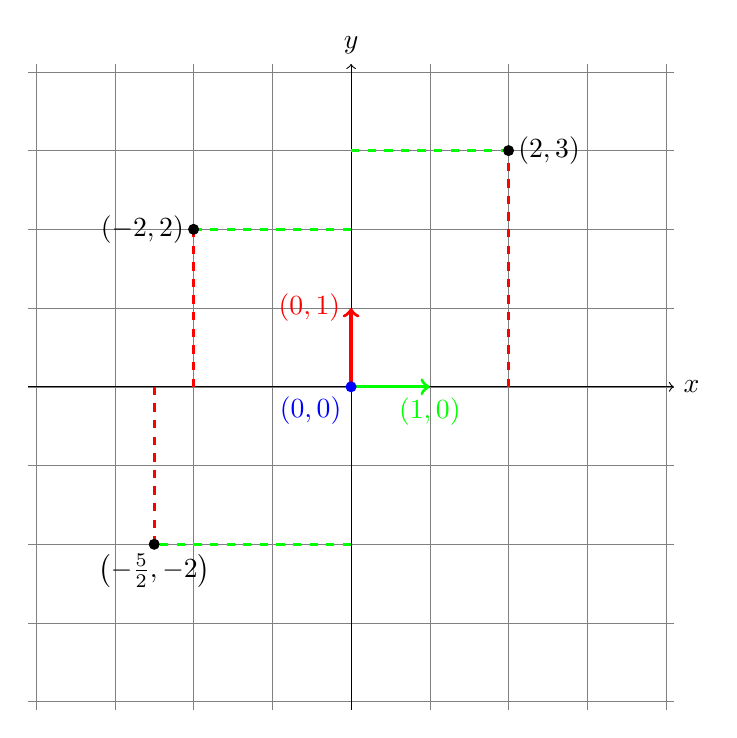
\begin{tikzpicture}
		\draw[help lines] (-4.1,-4.1) grid (4.1,4.1);
		\draw[->] (-4.1,0) -- (4.1,0) node[right]{$x$};
		\draw[->] (0,-4.1) -- (0,4.1) node[above]{$y$};
		\draw[green,very thick,->] (0,0) -- (1,0) node[below]{$(1,0)$};
		\draw[red,very thick,->] (0,0) -- (0,1) node[left]{$(0,1)$};
		\fill[blue] (0,0) circle(2pt) node[below left]{$(0,0)$};
		\draw[red,dashed,very thick] (2,0) -- (2,3);
		\draw[green,dashed,very thick] (0,3) -- (2,3);
		\fill (2,3) circle(2pt) node[right]{$(2,3)$};
		\draw[red,dashed,very thick] (-2,0) -- (-2,2);
		\draw[green,dashed,very thick] (0,2) -- (-2,2);
		\fill (-2,2) circle(2pt) node[left]{$(-2,2)$};
		\draw[red,dashed,very thick] (-5/2,0) -- (-5/2,-2);
		\draw[green,dashed,very thick] (0,-2) -- (-5/2,-2);
		\fill (-5/2,-2) circle(2pt) node[below]{$\left(-\frac{5}{2},-2\right)$};
	\end{tikzpicture}
\end{center}

\subsection{$\mathbb{R}^3$: El Espacio}

El mismo concepto se puede generalizar al espacio tridimensional, con tres ejes
que se juntan en el origen:

\begin{center}
	\begin{tikzpicture}[tdplot_main_coords]
		\draw[->] (-4,0,0) -- (4,0,0) node[right]{$x$};
		\draw[->] (0,-4,0) -- (0,4,0) node[above right]{$y$};
		\draw[->] (0,0,-4) -- (0,0,4) node[above]{$z$};
		\draw[green,very thick,->] (0,0,0) -- (1,0,0);
		\draw[red,very thick,->] (0,0,0) -- (0,1,0);
		\draw[purple,very thick,->] (0,0,0) -- (0,0,1);
		\fill[blue] circle(2pt);
		\draw[green,dashed,very thick] (0,3,0) -- (2,3,0);
		\draw[red,dashed,very thick] (2,0,0) -- (2,3,0);
		\draw[purple,dashed,very thick] (2,3,0) -- (2,3,1);
		\fill (2,3,1) circle(2pt) node[above]{$(2,3,1)$};
		\draw[green,dashed,very thick] (0,-2,0) -- (-3,-2,0);
		\draw[red,dashed,very thick] (-3,0,0) -- (-3,-2,0);
		\draw[purple,dashed,very thick] (-3,-2,0) -- (-3,-2,-2);
		\fill (-3,-2,-2) circle(2pt) node[below]{$(-3,-2,-2)$};
	\end{tikzpicture}
\end{center}

\end{document}
